\documentclass[11pt]{article}
\usepackage{geometry}                % See geometry.pdf to learn the layout options. There are lots.
\geometry{letterpaper}                   % ... or a4paper or a5paper or ... 
%\geometry{landscape}                % Activate for for rotated page geometry
%\usepackage[parfill]{parskip}    % Activate to begin paragraphs with an empty line rather than an indent
\usepackage{graphicx}
\usepackage{amssymb}
\usepackage{epstopdf}
\usepackage{url}
\usepackage{enumerate}

\DeclareGraphicsRule{.tif}{png}{.png}{`convert #1 `dirname #1`/`basename #1 .tif`.png}

\textheight = 8.5 in

\title{
\vspace{-20.mm}
CS57300: Homework 2}
\author{Due date: Wednesday February 18, midnight (submit pdf to Blackboard)}
\date{}                                           % Activate to display a given date or no date

\begin{document}
\maketitle
%\section{}
%\subsection{}

\vspace{-8.mm}
\noindent  \emph{Submit both your answers to the questions and the code that you used for analysis. Your homework must be typed. Use of Latex is recommended, but not required. }
\vspace{6.mm}

\noindent In this assignment, you will use R (and optionally python) to explore, transform, and analyze the Yelp data you started to use in HW1. Based on your analysis you will formulate hypotheses about the data. 


\section{Principal Component Analysis (6 pts)}

Consider the subset of the Yelp data comprised of the 35 numeric attributes.
\begin{enumerate}[(a)]
\item Run principal component analysis on the data. 
\item Plot the scree plot. Identify what number of components are needed to explain more than 95\% of the variance in the data. \\
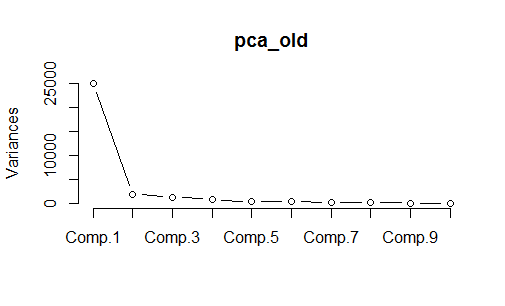
\includegraphics[width=4in]{pca_old.png}\\ 
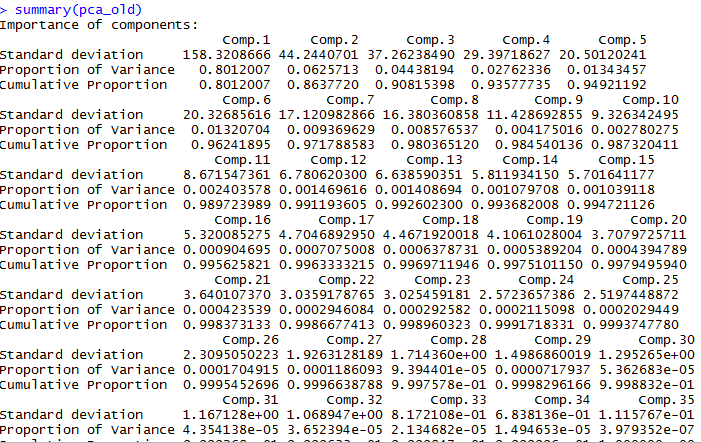
\includegraphics[width=4in]{pca_old_result.png}\\
We can conclude that 6 components are needed to explain 95\% of the variance.
\item Inspect the weights for the first principal component and identify how many of the 35 attributes have a significant weight in this component. \\
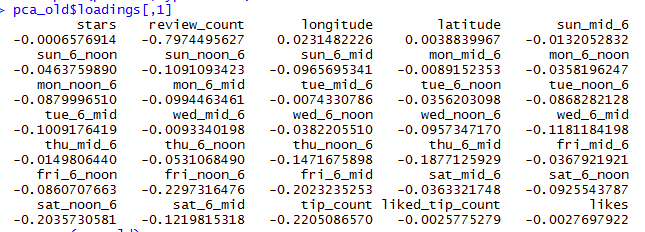
\includegraphics[width=4in]{a.png}\\
if we define significant weights is greater than 0.1, there are 11 attributes have significant weights.
\item Transform the data by removing the original column for {\em review\_count} and replace it with a new column containing log-transformed values of {\em review\_count}. Repeat the above analysis and discuss what if any changes you see in the results. \\
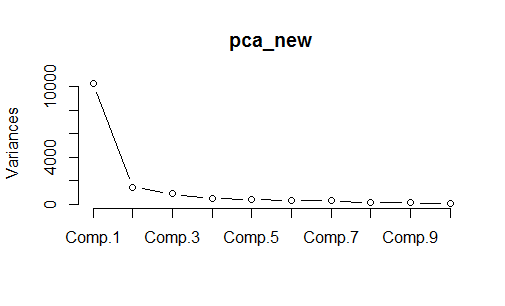
\includegraphics[width=4in]{pca_new.png}\\ 
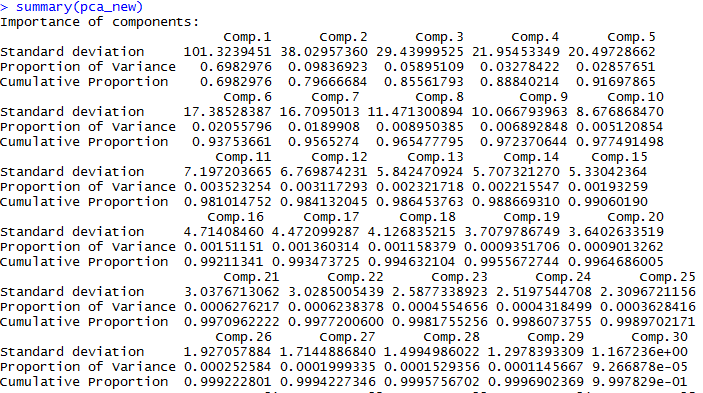
\includegraphics[width=4in]{pca_new_result.png}\\
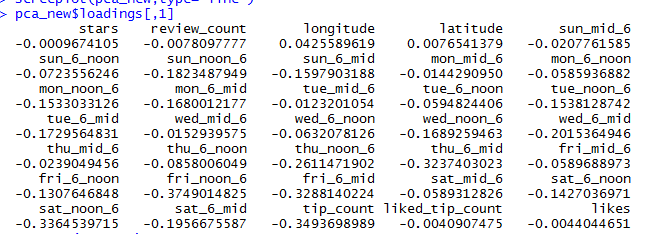
\includegraphics[width=4in]{b.png}\\
\\At this time, there are 7 components to explain 95\% of the variance and 17 attributes have significant weights. The change is that the {\em review\_count} doesn't dominant variance after using log value. The weight is change from 0.79 to 0.07. 
\item Sample a random set of 100 examples from the original data. Repeat the above analysis and discuss what if any changes you see in the results.
\begin{enumerate}
\item 
1 and 2\\
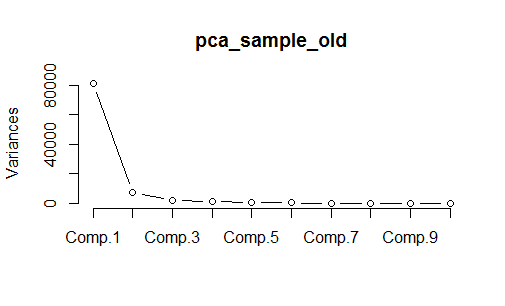
\includegraphics[width=4in]{pca_sample_old.png}\\
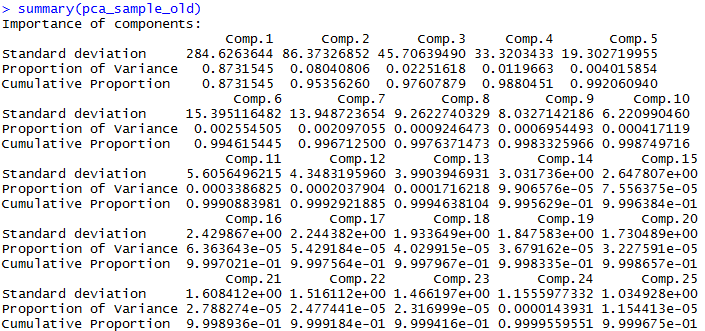
\includegraphics[width=4in]{c.png}\\
We can conclude that 2 components are needed to explain 95\% of the variance.
\item 3\\
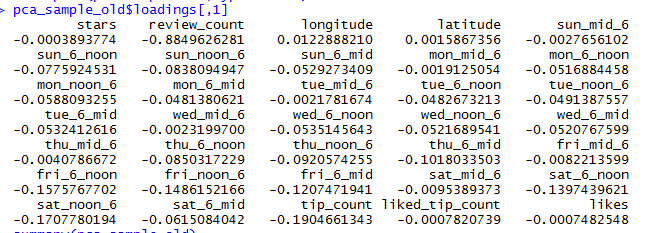
\includegraphics[width=4in]{d.png}\\
There are 7 attributes have significant weight.
\item 4\\
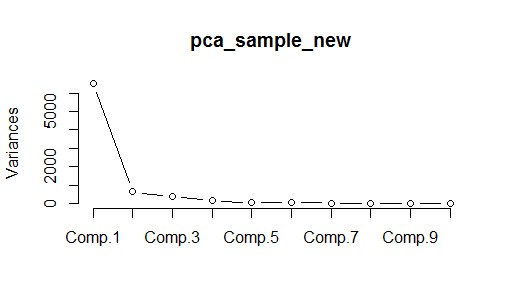
\includegraphics[width=4in]{pca_sample_new.png}\\
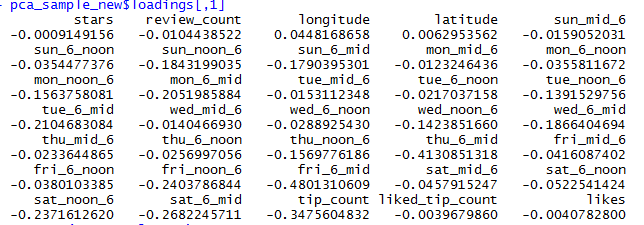
\includegraphics[width=4in]{e.png}\\
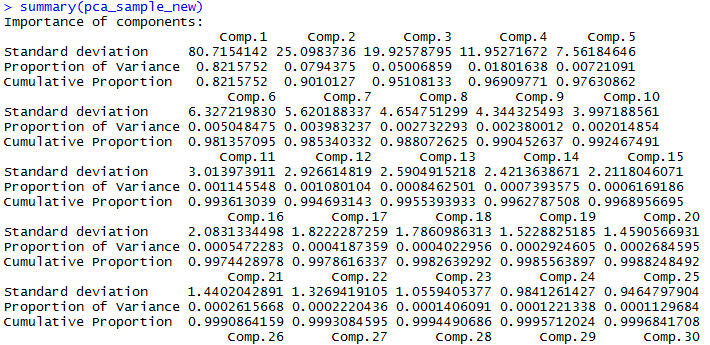
\includegraphics[width=4in]{f.png}\\
At this time, there are 4 components to explain 95\% of the variance and 15 attributes have significant weights. The change is that the {\em review\_count} doesn't dominant variance after using log value. The weight is change from 0.88 to 0.01. 
\\The sample result will take less components to explain most of difference.  
\end{enumerate} 
\end{enumerate}

\section{Scoring and search (12 pts)}
Consider the subset of the Yelp data with only the {\em review\_count} and {\em tip\_count} attributes.
\begin{enumerate}[(a)]
\item Run principal component analysis on the data. Report the eigenvector values (i.e., component weights) in the solution returned by R. \\
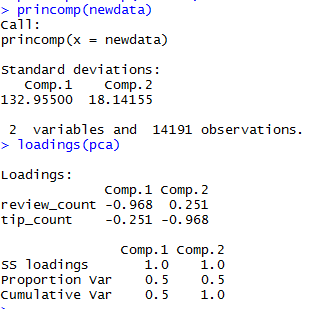
\includegraphics[width=4in]{score.png}\\
The eigen vactor values will be (-0.96,-0.251)
\item Develop your own algorithm to search over possible eigenvector solutions. \\
Recall that solutions must be orthogonal vectors of norm 1. Since the $p^{th}$ dimension is constrained by the solutions for the $[1,p-1]$ principal components, and your data for this question is 2-dimensional, you will only need to search for the values in first eigenvector. Moreover, since the eigenvector must have a norm of 1, you will only need to search over the first value for the eigenvector. 
\begin{itemize}
\item Mean center your data.
\item Consider a grid search over [-0.95,+0.95] with a step-size of 0.05 for the first eigenvector value (i.e., for {\em review\_count}, let's call this $v_1$). 
\item For each possible value of $v_1$, calculate a positive value for $v_2$ (i.e., for {\em tip\_count}) that constrains the vector $[v_1, v_2]$ to have a norm of 1. (Note that searching over positive and negative values for $v_1$ and only positive values for $v_2$ will cover all directions.)
\item For each choice of $[v_1, v_2]$, project the mean-centered data onto the vector and calculate the PCA score function (i.e., the variance of the projected data). 
\item Plot the score as a function of $v_1$ and identify the solution with the best score. Compare it to the solution returned by R and discuss any differences.\\
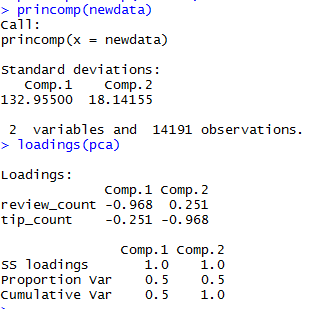
\includegraphics[width=4in]{score.png}\\
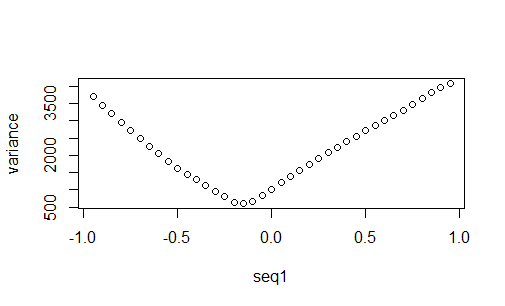
\includegraphics[width=4in]{basisvector.png}\\

According the graph, we can find that find the best score is at v1=0.95, which means the basis vector is at b=(0.95,0.312), close to result from pca by R. The difference is only the direction, but it doesn't matter. 

\end{itemize}
\end{enumerate}


\section{Transformations and associations (16 pts)} 

Consider the binary feature construction that you did in HW1 (e.g., Nightlife vs. not-Nightlife). In this question, you will construct binary features for values in the {\em category} and {\em city} attributes.

\begin{enumerate}[(a)]
\item Extract all the unique values in the {\em category} attribute by parsing the comma-separated lists (e.g., ``\texttt{Mexican, Restaurants}'' $\rightarrow$ two values, one for \texttt{Mexican} and one for \texttt{Restaurants}). Sort the list of values and choose the top 30. Construct binary features for each of these 30. (Note: you should figure out how to do this in a loop or a function, do not do it manually!)
\item Repeat the same process of binary feature construction for the {\em city} attribute, but this time use the top 30 most frequent cities in the data (i.e., reverse sort by number of examples in the city). Note: you do not need to parse this attribute.
\item For each pair of binary features ({\em category} vs. {\em city}; $30 \times 30$ pairs), determine whether there is any association by calculating $\chi^2$ scores (using \texttt{chisq.test}) from a contingency table of counts, e.g.:
\begin{table}[htdp] 
\begin{center}
\begin{tabular}{|c|c|c|}
\hline
& \multicolumn{2}{|c|}{City $i$}\\
 \hline
 Category $j$ &  0 & 1\\
 \hline
0 & ${N}_{00}$ & $N_{01}$ \\
 1 & $N_{10}$ & $N_{11}$ \\
\hline
\end{tabular}
\end{center}
\label{default}
\end{table}%

Report the top five features combinations with the largest $\chi^2$ scores, along with assessments of significance (i.e., $p$ values), and discuss whether the correlations are interesting or expected, given your domain knowledge. \\

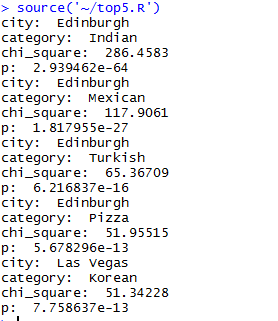
\includegraphics[width=2in]{top5.png}\\
According the result, we can conclude that Edinburgh has many food restaurant. Among the top 5 pairs, 4 of them is city Edinburgh.

\item Consider the feature pair with largest $\chi^2$ score (let's call this pair $A^{max}$) and another feature pair with a score that is barely significant (i.e., $A^{good}$ with $p$-value $\approx 0.05$). Investigate the effect of sampling on the scores of these feature pairs.
\begin{itemize}
\item Repeat ten times:
\begin{itemize}
\item Create ten random samples of the following sizes: \\ $[16, 32, 64, 128, 256, 512, 1024, 2048, 4096, 8192]$. 
\item Calculate the $\chi^2$ scores for $A^{max}$ and $A^{good}$ on each sample.
\end{itemize}
\item Calculate the mean and standard deviation of the scores for each feature pair, for each sample size.
\item Plot the $\chi^2$ scores as a function of sample size. Your plot should include one curve for $A^{max}$ and one curve for $A^{good}$ and include error bars to show the standard deviation.
\item Discuss the results. What effect does sample size have on significance? Does the effect vary across the two attributes?\\

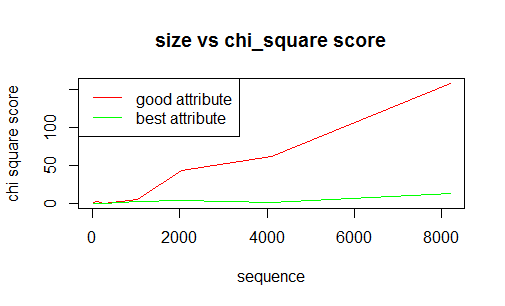
\includegraphics[width=5in]{chisquare.png}\\
The chi square is from 0 to 9.4 for good attribute and  form 0 to 149 for best attribute pair. According chart, we can conclude that the chi square will be more significant as the size of sample increased. The effect is similar across two attribute.

\end{itemize}

\end{enumerate}

\section{Identifying hypotheses (6 pts)}

The {\em stars} attribute corresponds to a rating for the business. The {\em review count} attribute records the number of reviews/ratings that the business received. Investigate how the binary features you created for the {\em city} and {\em categories} attributes, as well as the {\em latitude}, and {\em longitude} attributes relate to these two {\em stars} and {\em review count} attributes. Identify two hypotheses about the relationships between the features (one for {\em stars} and one for {\em review count}). For each of your hypotheses:
\begin{enumerate}[(a)]
\item Identify the type of hypothesis (descriptive vs. relational vs. causal; direction vs. non-directional).
\item State the hypothesis and discuss how your analysis of the data led you to the conjecture.
\item Include a plot to support your hypothesis.
%\item Subsample the data so that it only contains businesses with more than ten reviews and repeat your analysis. Discuss how this affects (or does not affect) the claims you've made about the data. %You can use the \texttt{subset()} function or select from the data frame with \texttt{[ ]} operations. 

\begin{enumerate}
\item
Type:Directional relational\\
Hypothesis: The average stars of Las Vegas restaurant is similar to the average stars of Phoenix restaurant\\
How: Getting all Las Vegas and Phoenix restaurants' stars and take average\\
Chart:\\
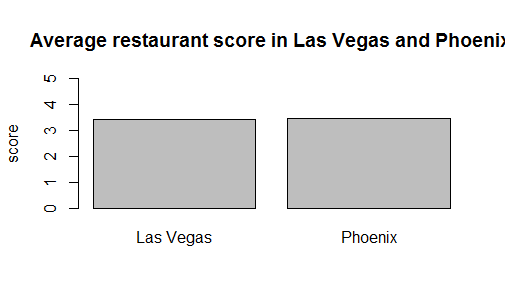
\includegraphics[width=5in]{lvphoenix.png}

\item
Type:Directional relational\\
Hypothesis: The average review count of Indian food is higher than Chinese food\\
How: Getting all Indian and Chinese restaurants' review count and take average\\
Chart:\\
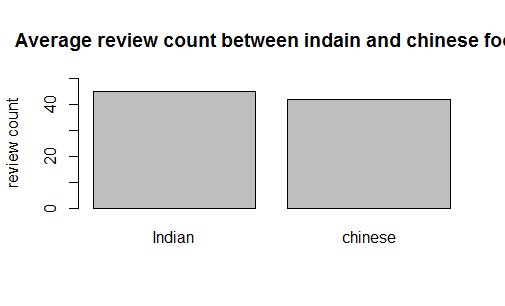
\includegraphics[width=5in]{review_count.png}
\end{enumerate}


\end{enumerate}


\end{document}  